% !TeX program = lualatex
% !TeX encoding = utf8
% !TeX spellcheck = uk_UA
% !TeX root =../FTProblems.tex

%=========================================================
\Opensolutionfile{answer}[\currfilebase/\currfilebase-Answers]
\Writetofile{answer}{\protect\section*{\nameref*{\currfilebase}}}
\chapter{Діелектрики та магнетики в статичних полях}\label{\currfilebase}
%=========================================================

\begin{Theory}[Основна задача електростатики]
	За наявності діелектриків, основна задача електростатики зводиться до розв'язання узагальненого рівняння Пуассона:
	\begin{equation}\label{eq:Gen_Poisson}
		\vect{\nabla} \cdot \left[ {\epsilon(\vect{r})\nabla {\pot}} \right] =  - 4\pi \rho(\vect{r}).
	\end{equation}
	з певними граничними умовами.

	\textbf{Формулювання задачі за наявності двох середовищ}.

\begin{wrapfigure}{l}{0.35\linewidth}
		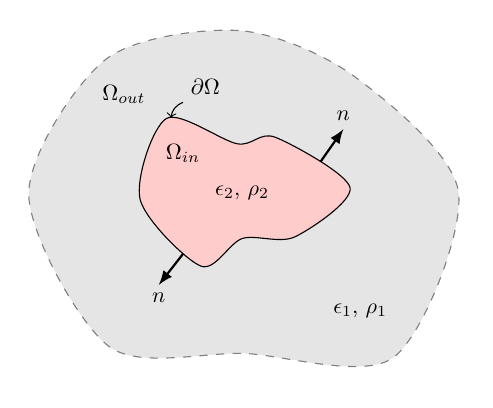
\begin{tikzpicture}[scale=0.5, every node/.style={scale=0.8}]
			\pgfmathsetseed{5}
			%        \draw (-3,-3) rectangle (3,3);
			\draw[fill=gray!20, draw=gray, dashed] plot [smooth cycle, samples=8,domain={1:8}] (\x*360/8+2*rnd:4cm+2cm*rnd);
			\pgfmathsetseed{10}
			\draw[fill=red!20] plot [smooth cycle, samples=8,domain={1:8}] (\x*360/8+6*rnd:1cm+2cm*rnd) ;
			\node at (-3,2.5) {$\Omega_\text{out}$};
			\node at (3,-3) {$\epsilon_1$, $\rho_1$};
			\node at (-1.5,1) {$\Omega_\text{in}$};
			\node at (0,0) {$\epsilon_2$, $\rho_2$};
			\draw[-latex, thick] (2,0.8) -- ++(55:1) node[above] {$\vect{n}$};
			\draw[-latex, thick] (-1.5,-1.55) -- ++(-128:1) node[below] {$\vect{n}$};
			\draw[->] (-1.5,2.3) node[above right] {$\partial\Omega$} to[bend right] ++(-128:0.5) ;
		\end{tikzpicture}
		\caption{До пояснення основної задачі електростатики}
		\label{pic:main_elstat_problem}
\end{wrapfigure}


	Нехай задана нескінченна область простору $\Omega_\text{out}$ з діелектричною проникністю $\epsilon_1(\vect{r})$, яка містить розподілений заряд густиною $\rho_1(\vect{r})$, що оточує внутрішню область $\Omega_\text{in}$ з діелектричною проникністю $\epsilon_2(\vect{r})$ і розподілом заряду $\rho_2(\vect{r})$ гладкою поверхнею $\partial\Omega$ (функції $\epsilon_i(\vect{r})$ та $\rho_i(\vect{r})$ (де $i= 1,2$) --- гладкі) (див. рис~\ref{pic:main_elstat_problem}). Крім того, на межі розділу є заряд, розподілений з густиною $\sigma(\vect{r})$, де $\vect{r} \in \partial\Omega$. Нехай двічі диференційовні функції $\pot_1(\vect{r})$ та $\pot_2(\vect{r})$  є розв'язками рівнянь~\eqref{eq:Gen_Poisson}:
	\begin{equation}\label{eq:Gen_Poisson1}
		\vect{\nabla} \cdot \left[ {\epsilon_i(\vect{r})\nabla {\pot_i}} \right] =  - 4\pi \rho_i(\vect{r}), \quad i =1,2.
	\end{equation}
	На межі областей $\partial\Omega$  накладемо умови на потенціали $\pot_1(\vect{r})$, $\pot_2(\vect{r})$:
	\begin{align}
		\left. \pot_1(\vect{r})\right|_{\vect{r}\in\partial\Omega}                                                                                                                                                                                              & =  \left.\pot_2(\vect{r})\right|_{\vect{r}\in\partial\Omega},        \\
		{\left. {\left( {{\epsilon _2}{\vect{n}} \cdot \vect{\nabla} {\pot_2}} \right)} \right|_{{\vect{r}} \in \partial \Omega }} - {\left. {\left( {{\epsilon _1}{\vect{n}} \cdot \vect{\nabla} {\pot_1}} \right)} \right|_{{\vect{r}} \in \partial \Omega }} & = {\left. {4\pi \sigma } \right|_{{\vect{r}} \in \partial \Omega }},
	\end{align}
	де $\vect{n}$~--- нормаль до поверхні $\partial\Omega$  з середовища $\Omega_\text{in}$   в середовище  $\Omega_\text{out}$.
	В області  $\Omega_\text{out}$ накладемо умову:
	\begin{equation}\label{}
		\lim\limits_{r \to \infty } \left\{ {\left| {\nabla {\pot _2}({\vect{r}})} \right|{r^2}} \right\} < \infty ,\quad r = \left| {\vect{r}} \right|,
	\end{equation}
	звідки випливає також, що $\lim\limits_{r \to \infty } \left\{ | \pot _2(\vect{r}) |r \right\} < \infty$.

	За умови виконання наведених умов,  розв'язок основної задачі електростатики визначається однозначно. Узагальнення на більшу кількість областей не призводить до складнощів. Якщо область $\Omega_\text{out}$ є обмеженою, то на її границі можна задати значення потенціалу (задача Діріхле). Якщо у системі є провідники, на їх поверхні додатково накладають умови аналогічні  мікроскопічному випадку.  За цих умов потенціали визначаються однозначно.
\end{Theory}


%=========================================================
\begin{problem}%
Діелектрична куля радіуса $R$  з проникністю  $\epsilon =\const > 1$ заряджена вільним зарядом $q$ , який розподілений однорідно по об’єму. Зовні ---
вакуум. Знайти розподіл потенціалу, електричної індукції та напруженості за допомогою інтегральної форми рівнянь Максвелла та нарисувати (схематично)
графіки залежності цих величин від радіальної змінної.
\end{problem}


%=========================================================
\begin{problem}%
Усередині нескінченного шару  $-a < x < a$  ($a> 0 $) об’ємна густина (вільного) заряду $\rho =
\const$ , діелектрична проникність $\epsilon =\const >
1$   (декартові координати). Зовні --- вакуум. Знайти (макроскопічну) напруженість та індукцію електричного поля, які створені зарядами шару.
\end{problem}


%=========================================================
\begin{problem}%
В однорідному середовищі діелектрична проникність  $\epsilon$. Знайти зв’язок між густиною вільних та зв’язаних зарядів.
\end{problem}

%=========================================================
\begin{problem}%
В однорідному статичному середовищі магнітна проникність $\mu$. Знайти зв’язок між густиною вільних струмів та струмів намагнічення.
\end{problem}



%=========================================================
\begin{problem}
    На плоскій поверхні, що розділяє середовища $1$ та $2$, задана поверхнева густина вільного заряду $\sigma$. У середовищах діелектричні проникності, відповідно, $\epsilon_1 > 1$ та $\epsilon_2 > 1$ . Нормаль $\vect{n}$ до поверхні спрямована з середовища $2$ в $1$. У середовищі $1$ задана напруженість електричного поля $\Efield_1$. Знайти напруженість електричного поля в середовищі $2$ у векторному вигляді.
\begin{solution}
    $\Efield_2 = \Efield_1 + \left( \frac{\epsilon_1}{\epsilon _2} - 1 \right)\vect{n}\left( \vect{n} \cdot \Efield_1 \right) - \frac{4\pi \sigma }{\epsilon _2}{\vect{n}}$.
\end{solution}
\end{problem}

%=========================================================
\begin{problem}
Точковий заряд $q$ розміщений на плоскій границі розділу двох однорідних  діелектриків (границю розділу вважати нескінченною) з проникностями $\epsilon_{1}$ і $\epsilon_{2}$. Знайти напруженість і індукцію електричного поля, а також його потенціал в усьому просторі.
\begin{solution}
	$
		\pot  = \frac{2}{{{\varepsilon _1} + {\varepsilon _2}}}\frac{q}{r},
	$
	$
		\Efield = \frac{2q}{\epsilon_1 + \epsilon_2}\frac{\vect{r}}{r^3},
	$
	$ \Dfield_i = \frac{2\epsilon_i}{\epsilon_1 + \epsilon_2}\frac{q\vect{r}}{r^3} $ ($i = 1,2$).
\end{solution}
\end{problem}


%=========================================================
\begin{problem}
Центр провідної кулі радіуса $R$  з зарядом $q$  розташований на плоскій межі розділу двох нескінченних однорідних діелектриків з проникностями $\epsilon_1$ та $\epsilon_2$ . Знайти потенціал та густину поверхневого заряду на кулі.
\begin{solution}
	Граничні умови на поверхні провідника $\pot = \const$  та межі розділу діелектриків можна задовольнити, використовуючи сферично-симетричний потенціал  $\pot(r) = \frac{C}{r}$, $r > R$ . Константу $C$ знаходимо з теореми Гаусса для індукції. Остаточно маємо потенціал:
	\[
		\pot(r) = \frac{2q}{(\epsilon_1 + \epsilon_2)r}, \quad r > R,
	\]
	та густину зарядів на поверхнях кулі:
	\[
		\sigma_i = \frac{q\epsilon_i}{2\pi(\epsilon_1 + \epsilon_2)R^2}, \quad i = 1,2.
	\]
\end{solution}
\end{problem}

%=========================================================
\begin{problem}
Усередині нескінченної провідної труби прямокутного перерізу $-a<x<a$; $-b<y<b$; $–\infty<z<\infty$,
усі бічні сторони якої заземлені, у площині $z=0$, вставлена тонка перетинка з поверхневою густиною
вільного заряду $\sigma  = \sigma _0\sin (\pi x/a)\sin (\pi y/b)$. Координати декартові. Діелектрична
проникність  $\epsilon (z < 0) = \epsilon _1$, $\epsilon (z > 0) = \epsilon _2$. Знайти розподіл
потенціалу $\pot(x,y,z)$ всередині труби.
\end{problem}

%=========================================================
\begin{problem}
На площині $z=0$ (декартові координати $x$,$y$,$z$) поверхнева густина вільного заряду
\begin{enumerate}[label=\alph*)]
	\item $\sigma (x,y) = \sigma _0\sin (\alpha x)\cos (\beta y)$;
	\item $\sigma (x,y) = {\sigma _0}{\sin ^2}(x/L)\cos (y/L)$.
\end{enumerate}
Діелектрична проникність  $\epsilon (z < 0) = \epsilon _1$, $\epsilon (z > 0) = \epsilon _2$. Знайти потенціал в усьому просторі.
\end{problem}

%=========================================================
\begin{problem}
Знайти силу, що діє на точковий сферично симетричний заряд  $q$ з боку незарядженої діелектричної
сфери радіусу $R$  з проникністю $\epsilon = \const$ . Відстань від заряду до центру сфери $D > R$.

\bigskip

\emph{Вказівка}: використати розклад потенціалу за поліномами Лежандра.
\end{problem}


%=========================================================
\begin{problem}
    Усередині однорідної діелектричної кулі радіусу $R$ з проникністю $\epsilon=\const$  об'ємна
    густина заряду в сферичних координатах  $\rho = \rho_0(r/R)^n\cos\theta$ ($r<R$). Куля оточена
    провідною сферою ($r = R$), яка заземлена. Знайти потенціал всередині кулі та густину зарядів,
    індукованих на сфері.
\end{problem}

%=========================================================
\begin{problem}
Провідну незаряджену заземлену кулю  радіуса $R$ вносять у зовнішнє однорідне електричне поле $\Efield_0$. Знайти індукований дипольний момент кулі  та розподіл індукованих зарядів на її поверхні.
\end{problem}

%=========================================================
\begin{problem}
Провідну заряджену ізольовану кулю (заряд $q$) радіуса $R$ вносять у зовнішнє однорідне електричне поле $\Efield_0$. Знайти індукований дипольний момент кулі  та розподіл індукованих зарядів на її поверхні.
\end{problem}

%=========================================================
\begin{problem}
Діелектричну кулю радіуса $R$ (діелектрична проникність кулі $\epsilon^{(i)}$) вносять у зовнішнє однорідне електричне поле з напруженістю $\Efield_0$ . Діелектрична проникність середовища навколо кулі дорівнює $\epsilon^{(e)}$. Знайти напруженість і потенціал поля в середині і зовні кулі. Знайти вектор поляризації кулі і густину зв'язаних зарядів на його поверхні.
\begin{solution}
	Зовні кулі на зовнішнє однорідне поле накладається поле, що створюється поляризаційними зарядами які виникли на кулі. З урахуванням нульової умови на нескінченності для поля зарядів на кулі та умови регулярності в початку координат, шукатимемо потенціал у вигляді:
	\[
		\pot(r) =
		\begin{cases}
			-Cr\cos\theta, \quad r \le R \\
			-E_0 r \cos\theta + \frac{p\cos\theta}{r^2}, \quad r > R.
		\end{cases}
	\]
	Граничні умови мають вигляд:
	\[
		\left. \pot^{(i)} \right|_{r = R} = \left. \pot^{(e)} \right|_{r = R} \left., \quad \epsilon^{(i)}\frac{\partial\pot^{(i)}}{\partial r}\right|_{r = R} =  \left. \epsilon^{(e)}\frac{\partial\pot^{(e)}}{\partial r}\right|_{r = R},
	\]
	і дають змогу визначити константу $C$ та дипольний момент $p$:
	\[
		\begin{cases}
			-CR\cos\theta = -E_0 R \cos\theta + \frac{p\cos\theta}{R^2} \\
			\epsilon^{(i)}(-C\cos\theta) = \epsilon^{(e)} E_0 \cos\theta + \epsilon^{(e)}\frac{2p\cos\theta}{R^3}.
		\end{cases}
	\]
	Звідки:
	\[
		p = \frac{\epsilon^{(i)} - \epsilon^{(e)}}{\epsilon^{(i)} + 2\epsilon^{(e)}}R^3E_0,
	\]
	\[
		C = \frac{3\epsilon^{(e)}}{\epsilon^{(i)} + 2\epsilon^{(e)}}.
	\]
	Потенціал дорівнює:
	\[
		\pot =
		\begin{cases}
			-\frac{3\epsilon^{(e)}}{\epsilon^{(i)} + 2\epsilon^{(e)}}\left( \Efield_0\cdot \vect{r}\right), & r \le R \\
			-\left( \Efield_0\cdot \vect{r}\right) + \frac{\vect{p} \vect{r}}{r^3},                         & r > R.
		\end{cases}
	\]
	Густина зв'язаного заряду:
	\[
		\sigma_   \text{зв'яз} = P_{1n} - P_{2n} = \frac{1}{4\pi} \left( \left.\frac{\partial\pot^{(i)}}{\partial r}\right|_{r = R} -  \left. \frac{\partial\pot^{(e)}}{\partial r}\right|_{r = R} \right)  = \frac{3}{4\pi} \frac{\epsilon_i - \epsilon_e}{\epsilon_i + 2\epsilon_e} E_0\cos\theta.
	\]
\end{solution}
\end{problem}


%=========================================================
\begin{problem}
Електричне поле утворене розподілом вільних зарядів зовні кулі з діелектричною проникністю $\epsilon$ радіуса $R$, всередині зарядів немає. Знайти потенціал $\pot(r,\theta,\phi)$  (в сферичних координатах) при $r<R$, якщо на поверхні $\pot(R,\theta,\phi) = \pot_0\cos\theta$, а також густину зв'язаних зарядів на поверхні.
\begin{solution}
	\emph{Вказівка}: Шукаємо розв’язок рівняння Лапласа всередині кулі (в сферичних координатах)  у вигляді $\pot(r,\theta,\phi) = f(r)\cos\theta$. Маємо загальний розв'язок для  $f(r) = A\frac{r}{R} + B\left( \frac{R}{r}\right)^2$.  Константи знаходимо з умови регулярності в нулі та з граничної умови при  $r = R$. Густина зв’язаних зарядів визначається за формулою $\sigma = \vect{P}\cdot\vect{n}$.
\end{solution}
\end{problem}

%=========================================================
\begin{problem}
Електричне поле утворене розподілом зарядів усередині кулі з діелектричною проникністю $\epsilon$ радіуса $R$. Зовні кулі~--- вакуум,  зарядів немає. Знайти потенціал $\pot(r,\theta,\phi)$ (в сферичних координатах $r$,$\theta$,$\phi$) при $r>R$, якщо на поверхні $\pot(R,\theta,\phi) = \pot_0\cos\theta$.
\begin{solution}
	$\pot = \pot_0 \left( \frac{R}{r}\right)^2\cos\theta $.
\end{solution}
\end{problem}

%=========================================================
\begin{problem}\label{prb:OrtFunc}
Електричне поле утворене розподілом зарядів на поверхні кулі радіуса $R$, всередині і зовні зарядів немає. Усередині кулі діелектрична проникність $\epsilon$, зовні~--- вакуум. На поверхні електричний потенціал $\pot(R,\theta,\phi) = \pot_0\cos\theta$. Знайти потенціал  $\pot(r,\theta,\phi)$  зовні та усередині кулі (в сферичних координатах) та густину вільних зарядів на поверхні кулі.
\begin{solution}
	\emph{Вказівка}: Шукаємо розв’язок рівняння Лапласа всередині кулі (в сферичних координатах)  у вигляді $\pot(r,\theta,\phi) = f(r)\cos\theta$. Маємо загальний розв'язок для  $f(r) = A\frac{r}{R} + B\left( \frac{R}{r}\right)^2$.  Константи $A$ та $B$ в середині та зовні кулі різні. Знаходимо іх з нульової умови на нескінченності при $r>R$, умови регулярності та з граничної умови при  $r = R$. Густину вільного заряду знаходимо з граничної умови для нормальної компоненти індукції на поверхні кулі.
\end{solution}
\end{problem}

%=========================================================
\begin{problem}
Електричне поле утворене розподілом зарядів на поверхні циліндру радіуса $R$, інших зарядів немає. Усередині діелектрична проникність $\epsilon$, зовні~--- вакуум. На поверхні $\pot(R,z,\phi) = \pot_0\cos(m\phi)$. Знайти потенціал $\pot(r,\theta,\phi) $ (зовні та усередині циліндру, в циліндричних координатах) та густину вільних зарядів на поверхні циліндру (координати $r$, $z$, $\phi$ --- циліндричні).
\begin{solution}
	\(
		\pot(R,z,\phi) =
		\begin{cases}
			\pot _0\left( \frac{r}{R} \right)^m\cos (m\varphi), r < R \\
			\pot _0\left( \frac{R}{r} \right)^m\cos (m\varphi), r \ge R.
		\end{cases}
	\),
	\(
		\sigma_\text{вільн} = \frac{m(\varepsilon  + 1)}{4\pi }\cos (m\varphi ).
	\)
\end{solution}
\end{problem}

%=========================================================
\begin{problem}\label{prb:L}
Електричне поле утворене розподілом зарядів
\[
	\sigma(\theta, \phi) = \sum\limits_{n=0}^{\infty}\sum\limits_{m = -n}^ns_{mn}Y_{nm}(\theta, \phi)
\]
(де припускаємо, що ряд швидко збігається)  на поверхні кулі радіуса $R$, інших зарядів немає. Усередині кулі діелектрична проникність $\epsilon$, зовні~--- вакуум. Знайти потенціал  $\pot(r,\theta,\phi)$ (зовні та усередині кулі, в сферичних координатах  $r$, $\theta$, $\phi$).
\begin{solution}
	Розв'язок слід шукати окремо зовні кулі ($r >R$ ) та всередині ($r<R$). Користуючись повнотою системи сферичних функцій на сфері, шукаємо розв’язок у вигляді:
	\[
		\pot(r,\theta ,\varphi ) = \sum\limits_{n = 0}^\infty  {\sum\limits_{m =  - n}^n {{f_{nm}}(r){Y_{nm}}(\theta ,\varphi )} } .
	\]
	Підставимо це в рівняння Лапласа в сферичних координатах:
	\begin{equation}\label{Laplace_prb:L}
		\Delta \pot  \equiv \frac{1}{{{r^2}}}\frac{\partial }{{\partial r}}\left( {{r^2}\frac{{\partial \pot }}{{\partial r}}} \right) + \frac{1}{{{r^2}}}\hat \Lambda \psi  = 0,
	\end{equation}
	де \(\hat \Lambda {Y_{nm}} \equiv \frac{1}{{\sin \theta }}\frac{\partial }{{\partial \theta }}\left( {\sin \theta \frac{{\partial {Y_{nm}}}}{{\partial \theta }}} \right) + \frac{1}{{{{\sin }^2}\theta }}\frac{{{\partial ^2}{Y_{nm}}}}{{\partial {\varphi ^2}}} =  - n\left( {n + 1} \right){Y_{nm}}\left( {\theta ,\varphi } \right)\) .

	Звідси, з огляду на незалежність сферичних функцій з різними індексами і лінійність рівняння Лапласа по $\pot$  (принцип суперпозиції!), кожну складову потенціалу можна розглядати окремо. Маємо
	\[
		\frac{1}{{{r^2}}}\frac{\partial }{{\partial r}}\left( {{r^2}\frac{{\partial {f_{nm}}}}{{\partial r}}} \right) - \frac{{n\left( {n + 1} \right)}}{{{r^2}}}{f_{nm}}(r) = 0
	\]
	для усіх $n= 0,1,2,\ldots$ , і $m = -n, -(n-1), \ldots, 0, \ldots, n-1, n$  для кожного $n$.
	Загальний розв’язок рівняння~\eqref{Laplace_prb:L} є комбінацією степеневих функцій
	\begin{equation}\label{star_prb:L}
		f_{nm}(r) = A_{nm}{\left( {\frac{r}{R}} \right)^n} + {B_{nm}}{\left( {\frac{R}{r}} \right)^{n + 1}}
	\end{equation}

	Нормування на $R$ введено для зручності, константи $A_{nm}$ та $B_{nm}$~--- різні всередині і зовні кулі.
	Зовні кулі ($r >R$) поле обмеженої системи зарядів має прямувати до нуля на нескінченності, тому $A_{nm} = 0$,

	\begin{equation}\label{dstar_prb:L}
		\pot_\mathrm{out}(r,\theta ,\varphi ) = \sum\limits_{n = 0}^\infty  {\sum\limits_{m =  - n}^n {{B_{nm}}{{\left( {\frac{R}{r}} \right)}^{n + 1}}{Y_{nm}}(\theta ,\varphi )} }.
	\end{equation}

	Аналогічно розглядаємо розв’язок усередині кулі, де, однак, поле має бути регулярним в нулі (\emph{в центрі немає якихось точкових зарядів}); тому в~\eqref{star_prb:L} слід відкинути члени з від'ємними степенями змінної $r < R$ :
	\begin{equation}\label{ddstar_prb:L}
		\pot_\mathrm{in}(r,\theta ,\varphi ) = \sum\limits_{n = 0}^\infty  {\sum\limits_{m =  - n}^n {{{\tilde A}_{nm}}{{\left( {\frac{r}{R}} \right)}^n}{Y_{nm}}(\theta ,\varphi )} }
	\end{equation}
	Маємо дві граничні умови на поверхні кулі ($r = R$). Умову для тангенціальних компонент напруженості електричного поля в даній задачі можна замінити умовою неперервності потенціалу
	\[
		\pot_\mathrm{out}(R,\theta ,\varphi ) = {\pot_\mathrm{in}}(R,\theta ,\varphi ).
	\]
	Це дає  $\tilde{A}_{nm} = B_{mn}$.
	Друга гранична умова використовує нормальні компоненти індукції $D_n =  - \epsilon \vect{n} \cdot \vect{\nabla}\pot  =  - \epsilon \frac{\partial \pot }{\partial r}$ , вона дає
	\[
		- \left. {\frac{{\partial {\pot_\mathrm{out}}}}{{\partial r}}} \right|_{r = R} + \varepsilon {\left. {\frac{{\partial {\pot_\mathrm{in}}}}{{\partial r}}} \right|_{r = R}} = 4\pi \sum\limits_{n = 0}^\infty  {\sum\limits_{m =  - n}^n {{s_{nm}}{Y_{nm}}(\theta ,\varphi )} }.
	\]
	Підстановка~\eqref{dstar_prb:L}, \eqref{ddstar_prb:L} з урахуванням  $\tilde{A}_{nm} = B_{mn}$ визначає ці коефіцієнти:
	\[
		\left( n + 1 + n\varepsilon  \right)B_{nm} = 4\pi s_{nm}.
	\]
	Отже, остаточно маємо:
	\[
		\pot(r,\theta,\phi) =
		\begin{cases}
			4\pi \sum\limits_{n = 0}^\infty  {\sum\limits_{m =  - n}^n {\frac{{{s_{nm}}}}{{n + 1 + n\varepsilon }}{{\left( {\frac{r}{R}} \right)}^n}{Y_{nm}}(\theta ,\varphi )} } , \quad r < R \\
			4\pi \sum\limits_{n = 0}^\infty  {\sum\limits_{m =  - n}^n {\frac{{{s_{nm}}}}{{n + 1 + n\varepsilon }}{{\left( {\frac{R}{r}} \right)}^{n + 1}}{Y_{nm}}(\theta ,\varphi )} } , \quad r \ge R.
		\end{cases}
	\]

\end{solution}
\end{problem}

%=========================================================
\begin{problem}
Електричне поле утворене розподілом вільних зарядів на поверхні циліндру радіуса $R$ з густиною $\sigma (z,\varphi ) = \sigma _0\sin (m\varphi )$, інших зарядів немає. Усередині циліндру діелектрична проникність $\epsilon$, зовні~--- вакуум. Знайти потенціал $\pot(r,z,\phi)$ (зовні та усередині циліндру), в циліндричних координатах  та густину вільних зарядів на поверхні циліндру.
\end{problem}

%=========================================================
\begin{problem}
Електричне поле утворене розподілом зарядів $\sigma (\theta ,\varphi ) = {\sigma _0}\cos (\theta ) + \sigma _1$   на поверхні кулі радіуса $R$, інших зарядів немає. Усередині діелектрична проникність $\epsilon$, зовні~--- вакуум. Знайти потенціал  $\pot(r,\theta,\phi)$ в усьому просторі (в сферичних координатах ).
\end{problem}

%=========================================================
\begin{problem}
    На пласкій поверхні, що розділяє середовища $1$ та $2$, задана поверхнева густина вільного струму $\vect{i}$. У середовищах магнітні проникності, відповідно, $\mu_1 > 1$ та $\mu_2 > 1$ . Нормаль $\vect{n}$ до поверхні спрямована з середовища $2$ в $1$. У середовищі $1$ задана напруженість магнітного поля $\Hfield_1$. Знайти напруженість магнітного поля в середовищі $2$ у векторному вигляді.
\begin{solution}
    $\Hfield_2 = \Hfield_1 + \left( \frac{\mu_1}{\mu_2} - 1 \right)\vect{n}\left( \vect{n} \cdot \Hfield_1 \right) + \frac{4\pi}{c}\left[\vect{n}\times\vect{i}\right] $.
\end{solution}
\end{problem}

%=========================================================
\begin{problem}
Нескінченний прямолінійний циліндричний провідник радіуса $R$  з магнітною проникністю $\mu_1$  знаходиться в зовнішньому неоднорідному магнітному полі. Віссю провідника є вісь аплікат $ОZ$. Напруженість зовнішнього поля $H_x = H_0\frac{x}{R}$, $H_y = - H_0\frac{y}{R}$, $H_z = 0$ (координати декартові). Магнітна проникність середовища зовні провідника $\mu_2$. Знайти напруженість поля усередині та зовні провідника, та густину поверхневого струму намагнічення на поверхні провідника.
\end{problem}

%=========================================================
\begin{problem}
В нескінченому прямому циліндричному провідникові радіуса $R$ тече вільний струм з густиною $a/r$, де
$r$~--- відстань від осі провідника, $a = \const$, напрямок~--- по осі провідника. Усередині магнітна
проникність $\mu = \const$, зовні~--- вакуум. Знайти векторний потенціал струму $\vect{A}(r)$  з
точністю до константи всередині та зовні провідника. Калібрувальна умова $\vect{\nabla}\cdot\vect{A} =
0$.
\begin{solution}
	$
\vect{A}(r) =
\begin{cases}
-\mu a (r - R) \vect{e}_z, & r \leqslant R, \\
-\mu a R \ln \left( \dfrac{r}{R} \right) \vect{e}_z, & r > R.
\end{cases}
	$
\end{solution}
\end{problem}

%=========================================================
\begin{problem}
Струм  $\vect{j} = j_0 \vect{e}_z$ протікає вздовж нескінченного циліндру радіуса $R$. Зовні струмів
немає. Напрямок осі циліндра заданий одиничним вектором  $\vect{e}_z$. Знайти (з точністю до адитивної
константи) вектор-потенціал магнітного поля $\vect{A})$  в усьому просторі, калібрувальна умова
$\vect{\nabla}\cdot\vect{A} = 0$. Результат подати у векторному вигляді через вектори $\vect{r}$ та
$\vect{e}_z$ ($\vect{r} \perp \vect{e}_z$) . Усередині магнітна проникність $\mu = \const$  ,
зовні~--- вакуум.
\end{problem}

%\section{Метод електричних зображень}
%=========================================================
\begin{problem}
Точковий заряд $q$ знаходиться в середовищі з діелектричною проникністю $\epsilon_1$ на відстані $d$ від границі розділу рідких діелектриків. Діелектрична проникність другого діелектрика дорівнює $\epsilon_2$. Чому дорівнює сила, що діє на заряд? Від чого залежить напрямок цієї сили?
\begin{solution}
	$F = \frac{\epsilon_2 - \epsilon_1}{(\epsilon_2 + \epsilon_1)\epsilon_1} \frac{q}{4d^2}$.
\end{solution}
\end{problem}

%=========================================================
\begin{problem}\label{prb:dipole_in_field}
У вакуумі, на відстані $d$ від напівпростору, заповненого однорідним діелектриком з проникністю $\epsilon$, закріплений центр точкового жорсткого диполя з моментом $\vect{p}$. Паралельно межі півпростору прикладене однорідне зовнішнє електричне поле $\Efield$ (рис.~\ref{dipole_in_field}). Диполь може вільно обертатися в площині, паралельній до напрямку $\Efield$ і ортогонально до межі діелектрика. Знайти значення кута 𝛼 між напрямком векторів $\Efield$ і $\vect{p}$, яке відповідає стійкому положенню рівноваги.
\begin{solution}
	В діелектрику виникає зображення диполя, з моментом $\vect{p}' = -\vect{p}\frac{\epsilon - 1}{\epsilon + 1}$.

	Сумарний момент сил, що діє на диполь
    \[
        \left[\vect{p}\times\Efield\right] + \left[\vect{p}\times\left( \frac{3(\vect{p}'\vect{r})\vect{r}}{r^5} - \frac{\vect{p}'}{r^3} \right) \right] = 0
    \]
Звідси для положень рівноваги маємо $\alpha=0$ та $\alpha = \pi$ . При $\xi = \left|\frac{E}{\frac{\epsilon - 1}{\epsilon + 1} \frac38\frac{p}{d^3}}\right|<1$  також маємо $\alpha = \pi \pm \arccos\xi$.
Положення рівноваги $\alpha = 0$  є стійким. Положення рівноваги $\alpha = \pi$ є нестійким при при $\xi >1$ , але стає стійким при $\xi < 1$. Положення, що відповідають $\alpha = \pi \pm \arccos\xi$  при $\xi <1$, є нестійкими.
\end{solution}
\end{problem}

%=========================================================
\begin{figure}[h!]\centering
	%---------------------------------------------------------
		\begin{tikzpicture}%[scale=1.5]
			\draw[ultra thick] (-2,0) -- (2,0);
			\fill[gray!50] (-2,-1) rectangle (2,0);
			\node at (-1.5,-0.5) {$\epsilon$};
            \coordinate (A) at (0,2);
			\draw[-latex', thick, red] (A) +(-90+45:1) -- (A) -- ++(90+45:1) node[black, above] {$\vect{p}$};
			\draw[thin, dash dot] (A) -- ([xshift=0.7cm]A) coordinate[pos=0.8] (B);
			\draw[thin] (B) arc (0:90+45:0.55) node[pos=0.5, above] {$\alpha$};
			\draw[thin, dash dot] (A) -- node [right] {$d$} (A|-0,0);
			\draw[-latex] ([xshift=-2cm]A) -- node[below] {$\Efield$} ([xshift=-0.25cm]A) ;
		\end{tikzpicture}
		\caption{До задачі~\ref{prb:dipole_in_field}}
		\label{dipole_in_field}
	%---------------------------------------------------------
\end{figure}
%=========================================================

%=========================================================
\begin{problem}
Незаряджена металева сфера маси $m$ плаває в діелектричній рідини з проникністю $\epsilon$, занурившись в неї на одну чверть свого об'єму. До якого потенціалу слід зарядити сферу, щоб вона плавала зануреною в неї наполовину?
\begin{solution}
	$\phi = \sqrt{8mg/(\epsilon-1)}$.
\end{solution}
\end{problem}

%=========================================================
\begin{problem}
Однорідний ізотропний діелектрик з проникністю $\epsilon$ заповнює весь нижній півпростір. У вакуумі на відстані $d$ від його поверхні знаходиться точковий заряд $q$. Визначити поверхневу густину поляризаційних (зв'язаних) зарядів в довільній точці на межі розділу, а також повний зв'язаний заряд на поверхні діелектрика. Який результат вийде, при $\epsilon\to\infty$, який це має фізичний зміст?
\begin{solution}
	$\sigma_\text{зв'яз} = - \frac{\epsilon - 1}{\epsilon + 1} \frac{qd}{2\pi(x^2  +h^2)^{3/2}}$, де $x$~-- координата вздовж межі розділу, $q_\text{зв'яз} = - \frac{\epsilon - 1}{\epsilon + 1}q$.
\end{solution}
\end{problem}

%=========================================================
\begin{problem}%Журнал квант 2018, №5, стор. 9
Два точкових заряди $q_1$ та $q_2$ знаходиться на однакових відстанях $d$ від границі розділу двох рідких діелектриків з проникностями $\epsilon_1$ та $\epsilon_2$, відповідно. Знайдіть сили, що діють на кожен з зарядів. Проаналізуйте знак сил, що діють на заряди.
\begin{solution}
	$F_1 = \frac{\epsilon_1 - \epsilon_2}{(\epsilon_1 + \epsilon_2)\epsilon_1} \frac{q_1^2}{4d^2} + \frac{2}{\epsilon_1 + \epsilon_2} \frac{q_1q_2}{4d^2}$,
	$F_2 = \frac{\epsilon_2 - \epsilon_1}{(\epsilon_1 + \epsilon_2)\epsilon_2} \frac{q_2^2}{4d^2} + \frac{2}{\epsilon_1 + \epsilon_2} \frac{q_1q_2}{4d^2}$.
\end{solution}
\end{problem}




\Closesolutionfile{answer}

